%!TEX TS-program = xelatex
%!TEX encoding = UTF-8 Unicode
%!TEX root = 2022-GS-ARTICLE.tex
%----------------------------------------------------------------- LANGUAGES ---
\newcommand{\mylanguages}{italian} % in reverse order
%---------------------------------------------------------- TITLE & SUBTITLE ---
\newcommand{\mytitle}{Black Cube}
\newcommand{\mysubtitle}{Denaturalizzazione estremizzata, ambiente virtuale espanso, alienazione dalla dimensione umana}
%----------------------------------------------------------------- AUTHOR(s) ---
\newcommand{\authorone}{Giancarlo Bottalico}
\newcommand{\institutione}{Conservatorio di musica "N. Piccinni", Bari}
\newcommand{\emailone}{giancarlobottalico@gmail.com}
%-------------------------------------------------------------------------------
%-------------------------------------------------------------- STYLE GS2020 ---
%!TEX TS-program = xelatex
%!TEX encoding = UTF-8 Unicode
%!TEX root = 2022-GS-ARTICLE.tex
%-------------------------------- PACKAGES AND OTHER DOCUMENT CONFIGURATIONS ---
\documentclass[
	a4paper,
	twocolumn,
	twoside,
	%openright
]{article}
\usepackage[
	top=20mm,
	bottom=25mm,
	textwidth=17.2cm,
	columnsep=0.8cm,
	bindingoffset=1cm,
	%showframe
]{geometry}
\usepackage[T1]{fontenc}
\usepackage[\mylanguages]{babel}
\usepackage{csquotes}
\usepackage{animate}
%\usepackage{parskip}
\usepackage[style=authoryear-ibid,backend=biber]{biblatex}
\bibliography{includes/bibliography.bib}
\usepackage{dblfloatfix}
\usepackage{subfigure}
\usepackage[subfigure]{tocloft}
\advance\cftsecnumwidth 0.5em\relax
\advance\cftsubsecindent 0.5em\relax
\advance\cftsubsecnumwidth 0.5em\relax
\usepackage{graphicx}
\usepackage{wrapfig}
% \usepackage{epstopdf}
% \epstopdfsetup{update}
\usepackage[usenames]{color}
\usepackage{xcolor}
\usepackage{tikz}
\usetikzlibrary{shapes,
                through,
								calc,
								intersections,
								backgrounds,
                positioning}
\usepackage{tkz-euclide}
\usepackage{amssymb}
\usepackage[
  colorlinks=true,
  linkcolor=black,
	anchorcolor=black,
	citecolor=black,
	filecolor=black,
	menucolor=black,
	runcolor=black,
	urlcolor=black
	]{hyperref}
\usepackage{Alegreya}
\linespread{1.05}
\usepackage{
	fontspec,
	xltxtra,
	xunicode
	}
\usepackage{
	xfrac,
	unicode-math
	}

\defaultfontfeatures{Mapping=tex-text}
\setmonofont[
	Scale=MatchLowercase
	]{Andale Mono}
\setmathfont[
	Scale=MatchLowercase,
	Scale=1
	]{Libertinus Math}

\usepackage{microtype}

\usepackage[
	hang,
	small,
	labelfont=bf,
	up,
	textfont=it,
	up
	]{caption}
\usepackage{paralist} % For compact item lists
\usepackage{etoolbox} % Some tools: used for quote environment
\AtBeginEnvironment{quote}{\small}
\usepackage{titletoc}
\usepackage{titling} % Customizing the title section
\usepackage{booktabs} % Horizontal rules in tables
\usepackage{enumitem} % Customized lists
\setlist[itemize]{noitemsep} % Make itemize lists more compact
\usepackage{abstract} % Allows abstract customization
\renewcommand{\abstractnamefont}{\normalfont\bfseries} % Set the "Abstract" text to bold
\renewcommand{\abstracttextfont}{\normalfont\small\itshape} % Set the abstract itself to small italic text
\usepackage{titlesec} % Allows customization of titles
\usepackage{tocloft}
\renewcommand\thesection{\Roman{section}} % Roman numerals for the sections
\renewcommand\thesubsection{\Roman{subsection}} % roman numerals for subsections
\titleformat{\section}[block]{\Large}{\thesection.}{1em}{} % Change the look of the section titles
\titleformat{\subsection}[block]{\large}{\thesubsection.}{1em}{} % Change the look of the section titles
%------------------------------------------------------------- TITLE SECTION ---
\setlength{\droptitle}{-4\baselineskip} % Move the title up
\pretitle{\begin{center}\huge\bfseries} % Article title formatting
\posttitle{\end{center}} % Article title closing formatting
\title{\mytitle \\[0.1cm] \large{\emph{\mysubtitle}}} % Article title
\author{%
\textsc{\authorone}\\%
\normalsize \institutione \\ %
\normalsize \emailone %
% activate
% \and % duplicate these 4 lines if more
% \textsc{\authortwo} \\%
% \normalsize \institutiontwo \\ %
% \normalsize \emailtwo %
}
\date{} % Leave empty to omit a date

\usepackage{fancyhdr} % Headers and footers
\pagestyle{fancy} % All pages have headers and footers
\fancyhead{} % Blank out the default header
\fancyfoot{} % Blank out the default footer
\fancyhead[C]{\small Giancarlo Bottalico • Conservatorio "N. Piccinni"} % Custom header text
\fancyfoot[RO]{\small \today~ • w: \input{includes/words.txt} • c: \input{includes/char.txt} • p:~\thepage} % Custom footer text
\fancyfoot[LE]{\small p:~\thepage~ • c: \input{includes/char.txt} • w: \input{includes/words.txt} • \today} % Custom footer text

%-------------------------------------------------------------------------------
%-------------------------------------------------------------------------------
%	LISTINGS
%-------------------------------------------------------------------------------
%-------------------------------------------------------------------------------
\usepackage{listings}
% lstlistings setup
\definecolor{gsbg}{rgb}{0.98,0.98,0.98}

\lstset{%
  aboveskip=10pt,
	belowskip=5pt,
  language=C++,
  numbers=none,%left,%none,
  tabsize=4,
  %frame=single,
  breaklines=true,
  numberstyle=\tiny\ttfamily,
  backgroundcolor=\color{gsbg},
  basicstyle=\footnotesize\ttfamily,
  %commentstyle=\slshape\color{mylstcmt}, %\itshape,
  %frameround=tttt,
  columns=flexible, %fixed,
  showstringspaces=false,
  emptylines=2,
  inputencoding=utf8,
  extendedchars=true,
  literate=	{á}{{\'a}}1
			{à}{{\`a}}1
			{ä}{{\"a}}1
			{â}{{\^a}}1
			{é}{{\'e}}1
			{è}{{\`e}}1
			{ë}{{\"e}}1
			{ê}{{\^e}}1
			{ï}{{\"i}}1
			{î}{{\^i}}1
			{ö}{{\"o}}1
			{ô}{{\^o}}1
			{è}{{\`e}}1
			{ù}{{\`u}}1
			{û}{{\^u}}1
			{ç}{{\c{c}}}1
			{Ç}{{\c{C}}}1,
  emph={component, declare, environment, import, library, process},
  emph={[2]ffunction, fconstant, fvariable},
  emph={[3]button, checkbox, vslider, hslider, nentry, vgroup, hgroup, tgroup, vbargraph, hbargraph, attach},
  %emphstyle=\color{yotxt}, %\underline, %\bfseries,
  %morecomment=[s][\color{mylstdoc}]{<mdoc>}{</mdoc>},
  rulecolor=\color{black}
}

\usepackage[framemethod=tikz]{mdframed} % Allows defining custom boxed/framed environments

%-------------------------------------------------------------------------------
%--------------------------------------------------- INFORMATION ENVIRONMENT ---
%-------------------------------------------------------------------------------

% Usage:
% \begin{info}[optional title, defaults to "Info:"]
% 	contents
% 	\end{info}

\mdfdefinestyle{info}{%
	topline=false, bottomline=false,
	leftline=false, rightline=false,
	nobreak,
	singleextra={%
		\fill[black](P-|O)circle[radius=0.4em];
		\node at(P-|O){\color{white}\scriptsize\bf i};
		\draw[very thick](P-|O)++(0,-0.8em)--(O);%--(O-|P);
	}
}

% Define a custom environment for information
\newenvironment{info}[1][Info:]{ % Set the default title to "Info:"
	\medskip
	\begin{mdframed}[style=info]
		\footnotesize\noindent{\textbf{#1}}
}{
	\end{mdframed}
}

%-------------------------------------------------------------------------------
%----------------------------------------------------- BIOGRAFIA ENVIRONMENT ---
%-------------------------------------------------------------------------------

% Usage:
% \begin{bio}[optional title, defaults to "Info:"]
% 	contents
% 	\end{bio}

\mdfdefinestyle{bio}{%
	topline=false, bottomline=false,
	leftline=false, rightline=false,
	nobreak,
	singleextra={%
		\fill[black](P-|O)circle[radius=0.4em];
		\node at(P-|O){\color{white}\scriptsize\bf b};
		\draw[very thick](P-|O)++(0,-0.8em)--(O);%--(O-|P);
	}
}

% Define a custom environment for information
\newenvironment{bio}[1][Biografia:]{ % Set the default title to "Info:"
	\medskip
	\begin{mdframed}[style=bio]
		\noindent{\textbf{#1}}
}{
	\end{mdframed}
}

%-------------------------------------------------------------------------------
%------------------------------------------------------- WARNING ENVIRONMENT ---
%-------------------------------------------------------------------------------

% Usage:
% \begin{warn}[optional title, defaults to "Warning:"]
%	Contents
% \end{warn}

\mdfdefinestyle{warning}{
	topline=false, bottomline=false,
	leftline=false, rightline=false,
	nobreak,
	singleextra={%
		\draw(P-|O)++(-0.5em,0)node(tmp1){};
		\draw(P-|O)++(0.5em,0)node(tmp2){};
		\fill[black,rotate around={45:(P-|O)}](tmp1)rectangle(tmp2);
		\node at(P-|O){\color{white}\scriptsize\bf !};
		\draw[very thick](P-|O)++(0,-1em)--(O);%--(O-|P);
	}
}

% Define a custom environment for warning text
\newenvironment{warn}[1][Warning:]{ % Set the default warning to "Warning:"
	\medskip
	\begin{mdframed}[style=warning]
		\noindent{\textbf{#1}}
}{
	\end{mdframed}
}

%-------------------------------------------------------------------- ABSTRACT -
\renewcommand{\maketitlehookd}{%
\begin{abstract}
\noindent\input{includes/abstract.txt}
\end{abstract}
}

%------------------------------------------------------------ BEGIN DOCUMENT ---
\begin{document}
	\maketitle
	\thispagestyle{empty}
	%-------------------------------------------------------------------- ABSTRACT -
	% The abstract is an external txt file inside the includes folder
	%-------------------------------------------------------------------------------
	%the "*" semanthic wrote before title serve to not give an item number to each section or subsection
	
\section{L'idea}
Immagina una dimensione tanto \textbf{lontana} da avere leggi fisiche a noi incomprensibili, ma abbastanza \textbf{vicina} da poterci interagire direttamente. Immagina una dimensione nella quale è possibile tutto ciò che non lo è nella nostra dimensione natia. É estremamente complesso anche solo da idealizzare? Eppure si tratta di una \textbf{nostra creazione}, ma nessuno ha idea di come si muovano gli oggetti al suo interno.
	
	\subsection{Genesi}
	Siamo legati direttamente ad una sola dimensione, ovvero l'unica realtà che ci rende vivi e ci da forma. Ma con il progredire degli anni l'umanità sta smarrendo la concezione di realtà, creando dimensioni virtuali che stanno ingoiando la nostra natura.
	La \textbf{denaturalizzazione} è un fenomeno artificiale che porta a smontare le componenti di un oggetto per poterle riformulare singolarmente. Questo strumento è un tassello fondamentale nello sviluppo di realtà virtuali come i \textbf{videogiochi}: dimensioni fisiche non reali.
	Senza aver compreso la dimensione degli eventi reali, stiamo azzardando ad immergerci in realtà espanse alternative a quella nella quale viviamo, che non abbiamo ancora indagato a pieno.
	
	\begin{figure}[h] %il comando [h] serve a posizionare la figura in questo punto specifico del documento
		\begin{quote}
			\textit{Così, guidato dagli algoritmi, l'essere umano perde sempre più il proprio potere di agire, la propria autonomia. Si trova dinanzi ad un mondo che sfugge alla sua comprensione. Si attiene a decisioni algoritmiche che non riesce a capire fino in fondo, gli algoritmi diventano scatole nere}
		\end{quote}
		\caption{Byung - Chul Han, "Le non cose", 2022}
	\end{figure}
	
	Ma Black Cube va persino oltre tutto questo. L'opera è un'estremizzazione del concetto di denaturalizzazione: l'obiettivo è creare una terza realtà fisica alternativa nella quale persino le nostre realtà aumentate vengono denaturalizzate e portate ad un livello più profondo di virtualità e di denaturalizzazione.
	Con quest'opera intendo dunque creare una realtà alternativa alla realtà alternativa denaturalizzandone ulteriormente l'astrazione, nella quale ogni gesto funzionale alle sue leggi fisiche diventa un gesto compositivo: l'unico linguaggio in grado di mettere in comunicazione questa terza dimensione difficilmente accessibile con la nostra concreta realtà è la musica.
	L'opera infatti è un'installazione musicale interattiva che attribuisce al giocatore la facoltà di compositore e fruitore della stessa, senza che neanche possa rendersene conto.
	L'intento è evidenziare lo smarrimento al quale andiamo in contro, l'allontanamento dalla nostra dimensione natia, di conseguenza fornire uno strumento per comprendere ciò che non controlliamo, per dettare le regole del gioco: la musica.
	
	\subsection{Interazione}
	Snocciolando questa terza dimensione, naturalmente emergono dei quesiti, tra i quali: in che modo questo videogioco gestisce l'estremizzazione della denaturalizzazione? In cosa consiste questa dimensione espansa? Come può il fruitore dell'opera diventare il compositore della musica che ne detta le regole fisiche? In che modo  l'opera rappresenta l'allontanamento dalla nostra reale dimensione?
	L'essenza dell'opera sta nell'implementazione dell'audio: il sound design è realizzato in maniera alternativa rispetto a quella tradizionale, creando suoni che interagiscano con i gesti del giocatore per astrazione più che per causalità. Gli eventi sono denaturalizzati: distaccano il gesto dell'oggetto sonoro dal suono riprodotto.
	Si tratta di un gioco di aspettative: al compimento di un gesto vengono generati dei suoni elettroacustici che "normalmente" non corrispondono ai suoni generati in un videogioco (quindi nella seconda dimensione: la realtà virtuale). Si creano dunque impulsi nervosi e sfuggenti dai gesti morbidi e dilatati, oppure suoni con lungo tempo di attacco e di decadimento dai gesti semplici e rapidi: i suoni e la musica non soddisfano dunque le aspettative del giocatore, perchè sembrano rispondere a delle leggi fisiche a noi sconosciute, appartenenti ad una realtà alternativa persino a quella virtuale.
	Un altro fattore risultante del gioco è il fine: il gioco non ha una misione, un obiettivo o un boss finale come nella "tradizionale" realtà virtuale: questo fattore simboleggia alla perfezione lo smarrimento, la mancanza di una meta o di una rotta da seguire, l'incomprensione della dimensione nella quale ci si trova

\section{L'OPERA}
Nei seguenti paragrafi entrerò nel merito della realizzazione concreta dell'opera, descrivendo ogni passaggio volto alla creazione della creazione dello spazio fisico e virtuale di Black Cube

	\subsection{Spazio Virtuale}
	Gli script di game engine di Black Cube sono scritti in C++. I soundbank per l'implementazione audio sono generati dal middleware Wwise. Di seguito la gerarchia degli eventi e delle azioni del gioco. Ciascuna con un proprio trigger che richiama un file audio, i quali vengono interpolati randomicamente ad ogni trigger in più parametri quali: pitch, gain, Eq(LowPass filter e HighPass filter), Flanging(Feedback, dry/wet). In modo tale che suonino sempre diversamente, rendendo l'esperienza esclusiva ad ogni singola azione del giocatore.
	Come si può vedere nella figura 2, gli eventi all'interno del soundbank "Main" sono organizzati in diverse sezioni, quali:
	\begin{compactitem}
		\item Items: suoni associati agli eventi delle diverse scene
		\item Magic: suoni associati alle armi magiche del main character
		\item Main Character: suoni associati alle azioni fisiche del giocatore
		\item Monsters: suoni associati alle azioni fisiche dei nemici
	\end{compactitem}
	
	\begin{figure}[h]
		\begin{center}
			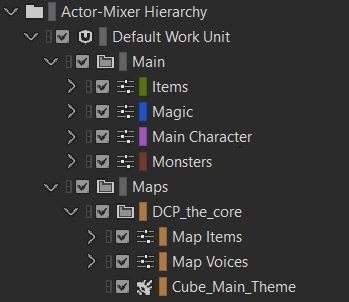
\includegraphics[width=.47\textwidth]{img/image2.jpg}
			\caption{\textbf{Gerarchia degli eventi all'interno dei soundbanks "Main" e "Maps"}}
			\label{gr01}
		\end{center}
	\end{figure}

	\begin{figure}[h]
		\begin{center}
			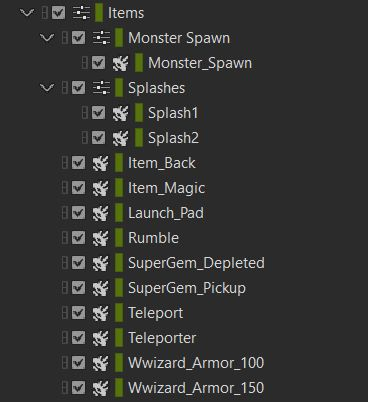
\includegraphics[width=.47\textwidth]{img/image3.jpg}
			\caption{\textbf{Gerarchia degli eventi sonori delle scene}}
			\label{gr01}
		\end{center}
	\end{figure}
	
	\begin{figure}[h]
		\begin{center}
			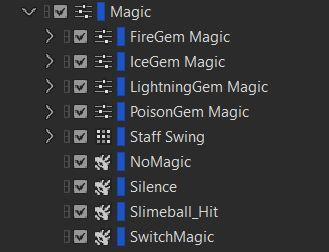
\includegraphics[width=.47\textwidth]{img/image4.jpg}
			\caption{\textbf{Gerarchia degli eventi sonori delle armi del giocatore}}
			\label{gr01}
		\end{center}
	\end{figure}

	\begin{figure}[h]
		\begin{center}
			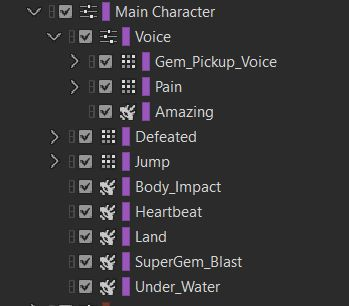
\includegraphics[width=.47\textwidth]{img/image5.jpg}
			\caption{\textbf{Gerarchia degli eventi sonori delle azioni fisiche del giocatore}}
			\label{gr01}
		\end{center}
	\end{figure}
	
	\begin{figure}[h]
		\begin{center}
			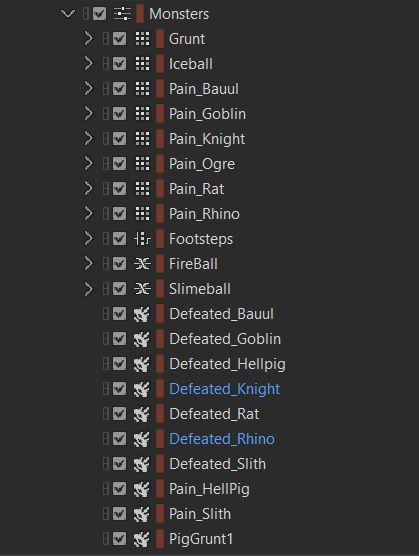
\includegraphics[width=.47\textwidth]{img/image6.jpg}
			\caption{\textbf{Gerarchia degli eventi sonori delle azioni fisiche dei nemici}}
				\label{gr01}
		\end{center}
	\end{figure}
	
	Si può notare che sono presenti diverse icone grafiche associate a ciascun evento. Questi simboli indicano il tipo di evento che viene richiamato per l'azione compiuta nel gioco. I principali sono:
	
	\begin{compactitem}
		\item Simple Event: questo è il più semplice trigger utilizzabile in Wwise. Rappresenta un evento audio che viene riprodotto una volta richiamato.
		\item Random Container: un insieme di eventi audio che vengono richiamati in maniera randomica ad ogni trigger. utilizzato ad esempio per i footsteps o per i jump sounds
		\item Switch Container: Utilizzato quando si desidera selezionare diversi eventi audio in base ad uno switch. il quale potrebbe corrispondere a una situazione di gioco specifica: uno stato.
		\item Blend Container: utilizzato per mescolare più eventi audio insieme, utile nelle transizioni. Utilizzato per alcune armi, laddove il loro utilizzo implica il trigger del lancio del proiettile e quello del suo impatto
		\item Sequence Container: Rriproduce gli eventi audio contenuti in sequenza, uno dopo l'altro, senza interruzioni.
	\end{compactitem}
	
	Alcuni di questi eventi sono modulati tramite RTPC (Real-Time Parameter Control). Si tratta di un sistema che consente di controllare i parametri sonori in tempo reale durante la riproduzione del gioco. 
	L'RTPC permette di modificare i valori di un parametro, come il volume o la frequenza di taglio di un filtro, in modo dinamico e in base a determinati eventi o situazioni all'interno del gioco. Ad esempio, si potrebbe utilizzare l'RTPC per aumentare il volume del gesto sonoro quando il giocatore si avvicina a una fonte di rumore, o per modificare la velocità di riproduzione della musica in base alla velocità di movimento del personaggio. In questo modo, è possibile creare un'esperienza sonora più immersiva e realistica per il giocatore.
	
	Il formato audio nel quale è stato missato il gioco è stereo a due canali. Nel calcolatore viene effettuato un routing interno dei segnali audio: l'audio in uscita dal videogioco viene mandato al canale virtuale del mixer Audient 1/2. Il fader del volume sarà impostato a -ifndB in modo che non esca dal master, il canale in questione viene impostato come fonte di Loopback. In un codice associato scritto in Maxmsp, l'audio viene prelevato dai canali 1/2 del mixer virtuale e processato secondo dei parametri descritti alla fine del paragrafo. L'audio in uscita di MaxMsp viene mandato ai canali 3/4 del mixer virtuale Audient, i quali vanno direttamente in uscita dal master. In questo modo ascolteremo solo l'audio in uscita da MaxMsp, che viene a sua volta prelevato da Black Cube.
	Il codice di MaxMsp ha lo scopo di restituire un feedback organico che si contrapponga all'astrazione: durante l'esperienza del giocatore, all'aumentare della sua immersione nella dimensione di Black Cube, dei suoni legati alla nostra dimensione, simboli di naturalezza e quotidianità, vengono richiamati dalla patch ammassandosi sempre di più con il passare del tempo e intensificandosi all'aumentare dell'escursione dinamica del gioco.
	Il soundscape generato dalla totalità dell'opera veicola la crescente necessità di ritorno alla nostra dimensione natia in seguito all'alienazione da questa data dall'esperienza immersiva in questo livello profondo di astrazione e virtualità. Maggiormente ci si smarrisce nella terza dimensione, maggiore è la necessità istintiva di evaderne e fare ritorno alla realtà.
	
	\subsection{Spazio Fisico}
	Ora estendiamo questa terza dimensione in uno spazio fisico appartenente alla nostra realtà. L'immersione in Black Cube prevede che il giocatore entri in una stanza rettangolare senza finestre, illuminata solo dalla luce dello schermo principale sul quale è proiettato Black Cube e dagli schermi laterali sui quali sono proiettate immagini della nostra dimensione, la cui luminosità aumenta all'aumentare  dell'escursione dinamica dei suoni organici generati dal codice.
	L'audio in uscita viene decodificato in ambisonics tramite una matrice sound field caricata all'interno del mixer fisico, le quattro uscite vengono inviate agli altoparlanti Front, Back, Left e Right
	
	\begin{figure}[h]
		\begin{center}
			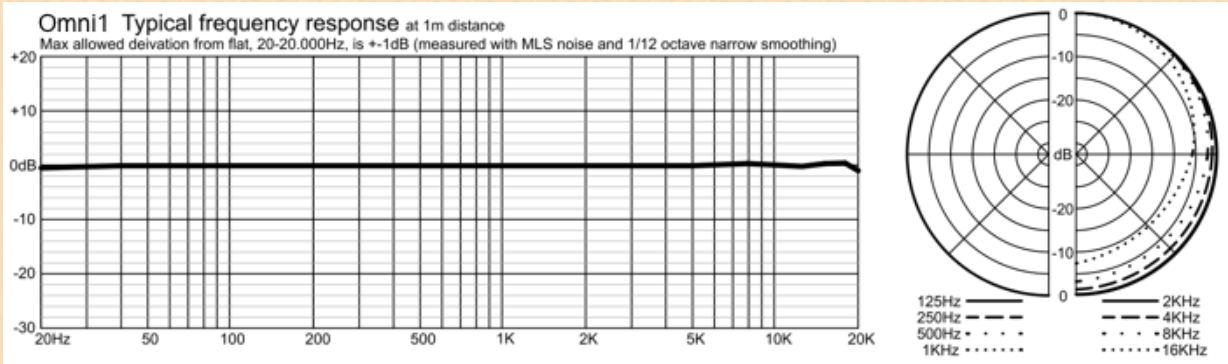
\includegraphics[width=10cm]{img/image1.png}
			\caption{\textbf{Modello 3D dello spazio fisico per l'allestimento dell'installazione}}
				\label{gr01}
		\end{center}
	\end{figure}

L'installazione è realizzata con un'approccio volto all'aumento dell'immersione del giocatore. L'obiettivo è fornire un'esperienza a 360° in grado di coinvolgere totalmente il fruitore dell'opera. Maggiore è il suo livello di immersione in Black Cube, maggiore è la comprensione dell'essenza dell'opera, il coinvolgimento emotivo e la sensibilizzazione che questa può dare al giocatore.
	
\section*{SVILUPPI ED APPLICAZIONI}
Tutto ciò trasforma Black Cube in un opera immersiva, coinvolgente, tattile. Ma che tipo di stimoli restituisce l'esperienza che offre? Cosa c'è da scoprire in un livello così profondo di astrazione e virtualtà? può Black Cube essere un'approccio suggestivo volto all'aumento delle capacità psichiche del giocatore? Può in qualche modo aumentare l'immersione e dunque il coinvolgimento del giocatore, sbloccandone un potenziale nascosto?

	\subsection*{Gamification}

	
	
	
	%I 10 microfoni sono stati organizzati in coppie stereofoniche AB, la quale prevede che essi siano distanziati ad una distanza variabile in base alle dimensioni della sorgente. In particolar modo:
	
	%\begin{enumerate}
	%	\item Una coppia per i primi violini e per le viole, posizionati specularmente nell'orchestra a distanza di 425cm l'uno dall'altro.
		
	%	\item Per la sezione dei fiati sono stati utilizzati tre microfoni, dei quali uno centrale e due laterali, per due motivi principali:
	%	\begin{compactitem}
	%		\item La sezione è molto ampia(428cm), dunque per evitare di avere un buco nella ripresa del centro della sezione, è stato aggiunto un microfono al centro del fronte.
	%		\item Per catturare anche i timpani, e in particolar modo il loro dettaglio timbrico, essendo storicamente utilizzati per dare sostegno ai fiati aggiungendo attacco e corpo al  suono.
	%	\end{compactitem}
		
	%	\item Una coppia a distanzata di 28cm per il pianoforte. Questa coppia è molto stretta rispetto alle altre perchè ha come intento quello di riprendere il pianoforte come oggetto centrale nell'immagine.
		
	%	\item Due utilizzati come Flanks, a distanza speculare di 324cm per allargare l'immagine stereo dell'ORTF. Il complesso Flanks + ORTF costituisce la ripresa MAIN dell'orchestra, ovvero quella generale, la quale serve a dare un'immagine complessiva frontale del corpo dell'orchestra e a riprendere l'interazione di quest'ultima con l'auditorium.
		
	%	\item Uno come spot per i contrabbassi, posto a 309cm dal flankR. La sua utilità sta nell'aggiungere il loro dettaglio alla ripresa complessiva. C'è da precisare che questo punto di ripresa non potrebbe dare informazioni sulla profondità della sezione trattandosi di un microfono mono, così come non potrebbe riprenderne fedelmente le basse frequenze essendo un microfono di spot e quindi molto vicino alla sorgente.
%	\end{enumerate}
	
	
	\vfill\null
	
	\newpage % USE NEWPAGE TO FORCE COLUMNN INTERRUPTION
	%-------------------------------------------------------------------------------
	%-------------------------------------------------------------------------------
	
	%--------------------------------------------
	%----------------larghezza massima del codice
	
	\vfill\null
	
	\raggedright
	%\bibliographystyle{unsrt}
	%\printbibliography
	
\end{document}

%%%%%%%%%%%%%%%%%%%%%%%%%%%%%%%%%%%%%%%%%%%%%%%%%%%%%%%%%%%%%%%%%%%%%%%%%%%%%%%%
% 2020 GIUSEPPE SILVI ARTICLE TEMPLATE BASED ON
%%%%%%%%%%%%%%%%%%%%%%%%%%%%%%%%%%%%%%%%%%%%%%%%%%%%%%%%%%%%%%%%%%%%%%%%%%%%%%%%
% Journal Article
% LaTeX Template
% Version 1.4 (15/5/16)
% This template has been downloaded from:
% http://www.LaTeXTemplates.com
% Original author:
% Frits Wenneker (http://www.howtotex.com) with extensive modifications by
% Vel (vel@LaTeXTemplates.com)
% License:
% CC BY-NC-SA 3.0 (http://creativecommons.org/licenses/by-nc-sa/3.0/)
%%%%%%%%%%%%%%%%%%%%%%%%%%%%%%%%%%%%%%%%%%%%%%%%%%%%%%%%%%%%%%%%%%%%%%%%%%%%%%%%
